\documentclass{article}

\usepackage{jacksonmath}
\usepackage[english]{babel}
\usepackage[utf8]{inputenc}
\usepackage[final]{pdfpages}

\begin{document}
  \section{Part I}
  \begin{enumerate}
    \item[4]
      Suppose that we let $\lambda=1$. I claim that this makes the set of solutions a vertical line.
      \begin{align}
        |z|=|z-1|\\
        x^2+y^2=(x-1)^2+y^2\\
        x^2+y^2=x^2-2x+1+y^2\\
        x=\frac{1}{2}
      \end{align}\qed
    \item[5]
      We have the equation $re(z+1)=|z-1|$. We can substitute $z=x+yi$ and get:
      \begin{align}
        x+1=\sqrt{(x-1)^2+y^2}\\
        (x+1)^2=(x-1)^2+y^2\\
        x^2+2x+1=x^2-2x+1+y^2\\
        x=\frac{y^2}{4}
      \end{align}
      I believe the line was intended to be $x=-1$ because the line should not intersect the parabola. Using this we can clearly see that this set of points are those that are equadistant from the line $x=-1$ and the point $(1,0)$.
    \item[6]
      \begin{enumerate}[label=\roman*]
        \item
          \includegraphics[scale=0.25]{extra/i.pdf}
        \item
          \includegraphics[scale=0.25]{extra/ii.pdf}
        \item
          \includegraphics[scale=0.25]{extra/iii.pdf}
        \item
          \includegraphics[scale=0.25]{extra/iv.pdf}
        \item
          \includegraphics[scale=0.25]{extra/v.pdf}
        \item
          \includegraphics[scale=0.25]{extra/vi.pdf}
        \item
          \includegraphics[scale=0.25]{extra/vii.pdf}
        \item
          \includegraphics[scale=0.25]{extra/viii.pdf}
      \end{enumerate}
    \item[8]
      First we will multiply these complex numbers together to get:
      \begin{align}
        zw&=rs(\cos\theta+i\sin\theta)(\cos\phi+i\sin\phi)\\
        &=rs(\cos\theta\cos\phi-\sin\theta\sin\phi+i(\cos\theta\sin\phi+\sin\theta\cos\phi))\\
        &=rs(\cos(\theta+\phi)+i\sin(\theta+\phi))
      \end{align}
      We can obviously see that:
      \begin{align}
        arg(zw)=\theta+\phi=arg(z)+arg(w)\tag{*}
      \end{align}
      Now we can try to prove DeMoivre's Theorem. The case where n=1 is obvious. Suppose n=2, and we will let $z=\cos\theta+i\sin\theta$. If we take $z^2$, by (3), we know \[z^2=\cos(2\theta)+i\sin(2\theta)\]
      Suppose this statement holds for $n$. Using (3) we can see:
      \begin{align*}
        z^n\cdot z=(\cos((n+1)\theta)+i\sin((n+1)\theta))
      \end{align*}
      Thus the statement holds for $n+1$, hence by induction
      \[(\cos\theta+i\sin\theta)^n=\cos n\theta+i\sin n\theta\]
    \item[12]
      \begin{align}
        \cos 5\theta+i\sin 5\theta&=\left(\cos ^5\left(x\right)-10\cos ^3\left(x\right)\sin ^2\left(x\right)+5\sin ^4\left(x\right)\cos \left(x\right)\right)\\&+i\left(5\cos ^4\left(x\right)\sin \left(x\right)-10\sin ^3\left(x\right)\cos ^2\left(x\right)+\sin ^5\left(x\right)\right)
      \end{align}
  \end{enumerate}
  \section{Part II}
  \begin{enumerate}
    \item[1]
      \begin{enumerate}[label=(\roman*)]
        \item $1<|z|<2$\\
          Let's first expand this to:
          \[1<x^2+y^2<2\] which is clearly the equation of a circle. It consists of all points that are inside a circle of radius 2 and outside the circle of radius 1. it is open.
          \\\includegraphics[scale=0.25]{extrag/i.png}
        \item $\re{z}\geq0$ and $\im{z}\leq \re{z}$\\
          The first part simple says that $x\geq0$. We can solve
          \[\im{z}\leq\re{z}\iff y\leq x\]
          and using these both we get the graph below. It is also a closed set.
          \\\includegraphics[scale=0.5]{extrag/ii.png}
        \item $\re{z}\geq0$ and $1<|z|<2$\\
          We know it is the points in the circle from (i) but with the additional condition that $x\geq0$. It is neither open nor closed because it does not contain all it's limit points and not every neighborhood is a subset of $\C$.\\
          \includegraphics[scale=0.5]{extrag/iii.png}
        \item $\re{zz_0}>0$\\
          First we need to find $\re{zz_0}$.
          \begin{align*}
            \re{z\cdot z_0}&=\re{(x+iy)(x_0+iy_0)}\\
            &=\re{xx_0-yy_0+(ixy_0+ix_0y)i}\\
            &=xx_0-yy_0\\
          \end{align*}
          Thus we have $xx_0>yy_0$. This presents us with three cases. The first is when $y_0>0$, this gives us $\frac{x_0}{y_0}x>y$. This is everything below the line with slope $\frac{x_0}{y_0}$. The case $y_0<0$ is similar to this case but shaded above the line.
          \\\includegraphics[scale=0.5]{extrag/ivs.png}\\
          Next we will let $y_0=0$. This case gives us $xx_0>0$. If we take some $x$, then this statement is true when sign$(xx_0)=1$, or sign$(x_0)x>0$. This set is open.
          \\\includegraphics[scale=0.5]{extrag/iv.png}\\
        \item $a<\arg(z-z_0)<b$ where $-\pi<a<b\leq\pi$\\
          Let the black and purple dotted lines represent the angles $a$ and $b$ respectively. Let's consider a point $z$. We want the line from $0$ to $z-z_0$ to have an angle between $a,b$. To make this easier let's shift this line by $z_0$ to get a line from $z_0$ to $z$ with an angle between $a,b$. Thus the set is the arc between $a,b$ but centered on $z_0$. This is true for any $z_0$. Because 0 is not a possible $z$ then this is open.
          \\\includegraphics[scale=0.3]{extrag/v.png}
        \item $|z-\bar{z_0}|=|\bar{z}-z_0|$\\
          We would expect these to always be equal because the complement just reflects over the x-axis. This set is $\C$ which is open and closed.
          \begin{align*}
            \sqrt{(x-x_0)^2+(y-(-y_0))^2}&=\sqrt{(x-x_0)^2+((-y)-y_0)^2}\\
            (x-x_0)^2+(y+y_0)^2&=(x-x_0)^2+(-(y+y_0))^2\\
            (y+y_0)^2&=(y+y_0)^2\\
            0&=0
          \end{align*}
          This statement is vacuously true for all $z$ and $z_0$
          \\\includegraphics[scale=0.5]{extrag/vi.png}
        \item $|z-\bar{z_0}|<|\bar{z}-z_0|$\\
          By similar work from last time.
          \begin{align*}
            \sqrt{(x-x_0)^2+(y-(-y_0))^2}&<\sqrt{(x-x_0)^2+((-y)-y_0)^2}\\
            (x-x_0)^2+(y+y_0)^2&<(x-x_0)^2+(-(y+y_0))^2\\
            (y+y_0)^2&<(y+y_0)^2\\
            0&<0
          \end{align*}
          Obviously there is no $z$ such that $0>0$. This set is $\emptyset$ which is open and closed
          \\\includegraphics[scale=0.5]{extrag/vii.png}
        \item $|z-\bar{z_0}|\leq|\bar{z}-z_0|$\\
          From (vi) and (vii) we need $0<0$ or $0=0$, this is vacuously true. This set is $\C$ so it is open and closed.
          \\\includegraphics[scale=0.5]{extrag/vi.png}
        \item $\re{z^2}>0$\\
          Let's first find $\re{z^2}$
          \[(x+iy)^2=x^2-y^2+2ixy\]
          So $x^2-y^2>0$ which simplifies to $|x|>|y|$ or $-|x|<y<|x|$. 0 is in the set but it does not have a neighborhood that is a subset so neither open nor closed.
          \\\includegraphics[scale=0.5]{extrag/ix.png}
        \item $\re{z^2}\leq0$\\
          This is similar to (ix). $-|x|\geq y\geq|x|$. closed
          \\\includegraphics[scale=0.5]{extrag/x.png}
        \item $\re{z^2}>1$\\
          We can solve this to $x^2-y^2>1$. This is the ``outside'' of a hyperbola. Open
          \\\includegraphics[scale=0.5]{extrag/xi.png}
        \item $\re{z^2}\leq1$\\
          This solves to $x^2-y^2\leq1$, which is the ``inside'' of a hyperbola. Closed
          \\\includegraphics[scale=0.5]{extrag/xii.png}
      \end{enumerate}
  \end{enumerate}
\end{document}
